%!TEX spellcheck
%%%%%%%%%%%%%%%%%%%%%%%%%%%%%%%%%%%%%%%%%
% Beamer Presentation
% LaTeX Template
% Version 2.0 (March 8, 2022)
%
% This template originates from:
% https://www.LaTeXTemplates.com
%
% Author:
% Vel (vel@latextemplates.com)
%
% License:
% CC BY-NC-SA 4.0 (https://creativecommons.org/licenses/by-nc-sa/4.0/)
%
%%%%%%%%%%%%%%%%%%%%%%%%%%%%%%%%%%%%%%%%%

%----------------------------------------------------------------------------------------
%	PACKAGES AND OTHER DOCUMENT CONFIGURATIONS
%----------------------------------------------------------------------------------------

\documentclass[
	11pt, % Set the default font size, options include: 8pt, 9pt, 10pt, 11pt, 12pt, 14pt, 17pt, 20pt
	%t, % Uncomment to vertically align all slide content to the top of the slide, rather than the default centered
	%aspectratio=169, % Uncomment to set the aspect ratio to a 16:9 ratio which matches the aspect ratio of 1080p and 4K screens and projectors
	% handout,
]{beamer}

\graphicspath{{Images/}{./}} % Specifies where to look for included images (trailing slash required)

\usepackage{booktabs} % Allows the use of \toprule, \midrule and \bottomrule for better rules in tables

%----------------------------------------------------------------------------------------
%	SELECT LAYOUT THEME
%----------------------------------------------------------------------------------------

% Beamer comes with a number of default layout themes which change the colors and layouts of slides. Below is a list of all themes available, uncomment each in turn to see what they look like.

%\usetheme{default}
%\usetheme{AnnArbor}
%\usetheme{Antibes}
%\usetheme{Bergen}
%\usetheme{Berkeley}
%\usetheme{Berlin}
%\usetheme{Boadilla}
%\usetheme{CambridgeUS}
%\usetheme{Copenhagen}
%\usetheme{Darmstadt}
%\usetheme{Dresden}
%\usetheme{Frankfurt}
%\usetheme{Goettingen}
%\usetheme{Hannover}
%\usetheme{Ilmenau}
%\usetheme{JuanLesPins}
%\usetheme{Luebeck}
\usetheme{Madrid}
%\usetheme{Malmoe}
%\usetheme{Marburg}
%\usetheme{Montpellier}
%\usetheme{PaloAlto}
%\usetheme{Pittsburgh}
%\usetheme{Rochester}
%\usetheme{Singapore}
%\usetheme{Szeged}
%\usetheme{Warsaw}


%----------------------------------------------------------------------------------------
%	SELECT COLOR THEME
%----------------------------------------------------------------------------------------

% Beamer comes with a number of color themes that can be applied to any layout theme to change its colors. Uncomment each of these in turn to see how they change the colors of your selected layout theme.

%\usecolortheme{albatross}
%\usecolortheme{beaver}
%\usecolortheme{beetle}
%\usecolortheme{crane}
%\usecolortheme{dolphin}
%\usecolortheme{dove}
%\usecolortheme{fly}
%\usecolortheme{lily}
%\usecolortheme{monarca}
%\usecolortheme{seagull}
%\usecolortheme{seahorse}
%\usecolortheme{spruce}
%\usecolortheme{whale}
%\usecolortheme{wolverine}

%----------------------------------------------------------------------------------------
%	SELECT FONT THEME & FONTS
%----------------------------------------------------------------------------------------

% Beamer comes with several font themes to easily change the fonts used in various parts of the presentation. Review the comments beside each one to decide if you would like to use it. Note that additional options can be specified for several of these font themes, consult the beamer documentation for more information.

\usefonttheme{default} % Typeset using the default sans serif font
%\usefonttheme{serif} % Typeset using the default serif font (make sure a sans font isn't being set as the default font if you use this option!)
%\usefonttheme{structurebold} % Typeset important structure text (titles, headlines, footlines, sidebar, etc) in bold
%\usefonttheme{structureitalicserif} % Typeset important structure text (titles, headlines, footlines, sidebar, etc) in italic serif
%\usefonttheme{structuresmallcapsserif} % Typeset important structure text (titles, headlines, footlines, sidebar, etc) in small caps serif

%------------------------------------------------

%\usepackage{mathptmx} % Use the Times font for serif text
\usepackage{palatino} % Use the Palatino font for serif text
\usepackage{hyperref}
%\usepackage{helvet} % Use the Helvetica font for sans serif text
\usepackage[default]{opensans} % Use the Open Sans font for sans serif text
%\usepackage[default]{FiraSans} % Use the Fira Sans font for sans serif text
%\usepackage[default]{lato} % Use the Lato font for sans serif text
\usepackage{ctex}
\usepackage{amsmath}

%----------------------------------------------------------------------------------------
%	SELECT INNER THEME
%----------------------------------------------------------------------------------------

% Inner themes change the styling of internal slide elements, for example: bullet points, blocks, bibliography entries, title pages, theorems, etc. Uncomment each theme in turn to see what changes it makes to your presentation.

%\useinnertheme{default}
\useinnertheme{circles}
%\useinnertheme{rectangles}
%\useinnertheme{rounded}
%\useinnertheme{inmargin}

%----------------------------------------------------------------------------------------
%	SELECT OUTER THEME
%----------------------------------------------------------------------------------------

% Outer themes change the overall layout of slides, such as: header and footer lines, sidebars and slide titles. Uncomment each theme in turn to see what changes it makes to your presentation.

%\useoutertheme{default}
%\useoutertheme{infolines}
%\useoutertheme{miniframes}
%\useoutertheme{smoothbars}
%\useoutertheme{sidebar}
%\useoutertheme{split}
%\useoutertheme{shadow}
%\useoutertheme{tree}
%\useoutertheme{smoothtree}

%\setbeamertemplate{footline} % Uncomment this line to remove the footer line in all slides
%\setbeamertemplate{footline}[page number] % Uncomment this line to replace the footer line in all slides with a simple slide count

%\setbeamertemplate{navigation symbols}{} % Uncomment this line to remove the navigation symbols from the bottom of all slides

%----------------------------------------------------------------------------------------
%	PRESENTATION INFORMATION
%----------------------------------------------------------------------------------------

\title[Arithmetic]{Arithmetic} % The short title in the optional parameter appears at the bottom of every slide, the full title in the main parameter is only on the title page

\subtitle{算术} % Presentation subtitle, remove this command if a subtitle isn't required

\author[张凡]{张凡} % Presenter name(s), the optional parameter can contain a shortened version to appear on the bottom of every slide, while the main parameter will appear on the title slide

\institute[XDF]{新东方国际教育 \\ \smallskip \textit{zhangfan@xdf.cn}} % Your institution, the optional parameter can be used for the institution shorthand and will appear on the bottom of every slide after author names, while the required parameter is used on the title slide and can include your email address or additional information on separate lines

\date[\today]{GRE 冲分班数学 \\ \today} % Presentation date or conference/meeting name, the optional parameter can contain a shortened version to appear on the bottom of every slide, while the required parameter value is output to the title slide

%----------------------------------------------------------------------------------------


%----------------------------------------------------------------------------------------
%	Section Slide
%----------------------------------------------------------------------------------------
\AtBeginSection[]{
  \begin{frame}
  \vfill
  \centering
  \begin{beamercolorbox}[sep=8pt,center,shadow=true,rounded=true]{title}
    \usebeamerfont{title}\insertsectionhead\par%
  \end{beamercolorbox}
  \vfill
  \end{frame}

	\begin{frame}
		\frametitle{Presentation Overview for \secname} % Slide title, remove this command for no title
		\tableofcontents[currentsection, hideothersubsections, sectionstyle=show/show]
	\end{frame}
  }



%----------------------------------------------------------------------------------------

\AtBeginSubsection[]{
  \begin{frame}
  \vfill
  \centering
    \usebeamerfont{title}\insertsubsectionhead\par%
  \vfill
  \end{frame}
}
%----------------------------------------------------------------------------------------


\begin{document}

%----------------------------------------------------------------------------------------
%	TITLE SLIDE
%----------------------------------------------------------------------------------------

\begin{frame}
	\titlepage % Output the title slide, automatically created using the text entered in the PRESENTATION INFORMATION block above
\end{frame}

%----------------------------------------------------------------------------------------
%	TABLE OF CONTENTS SLIDE
%----------------------------------------------------------------------------------------

% The table of contents outputs the sections and subsections that appear in your presentation, specified with the standard \section and \subsection commands. You may either display all sections and subsections on one slide with \tableofcontents, or display each section at a time on subsequent slides with \tableofcontents[pausesections]. The latter is useful if you want to step through each section and mention what you will discuss.


%----------------------------------------------------------------------------------------
%	PRESENTATION BODY SLIDES
%----------------------------------------------------------------------------------------
\begin{frame}
	\frametitle{To Begin With}
	\begin{block}{QR Mathematical Convention 1 }
		Any number in QR is a real number. \\ Imaginary Numbers are \alert{out of scope of} QR.
	\end{block}
\end{frame}
%------------------------------------------------



\section{Integers}

\subsection{Even v.s. Odd}

%------------------------------------------------

\begin{frame}
	\frametitle{The Big Question}

	{\LARGE Can negative numbers be odd or even? \\ For example, is -2 Even?\\ }
	\pause
	\bigskip
	{\LARGE \textbf{\alert{YES!}}}
\end{frame}

%------------------------------------------------

\begin{frame}
	\frametitle{Even v.s. Odd}
	\framesubtitle{奇偶运算: 看剩下的尾巴}
		\begin{definition}
		  x is an odd number  if $x = 2k + 1$, where $\alert{k = .... -2, -1, 0, 1, 2, ...}$.\\
		  x is an even number  if $x = 2k$, where $\alert{k = .... -2, -1, 0, 1, 2, ...}$.
	 \end{definition}
	
	\smallskip % Vertical whitespace

	\begin{block}{Facts about Odd and Even Numbers}
			\begin{itemize}
			\item $odd \pm even = odd$  \quad $(2k_1 + 1) \pm 2k_2 = 2(k_1 \pm k_2) + \textbf{\alert{1}}$
			\item $odd \pm odd = even$ \quad $(2k_1 + 1) \pm (2k_2 + 1) = 2(k_1 \pm k_2) $
			\item $even \pm even = even$ \quad $2k_1  \pm 2k_2  = 2(k_1 \pm k_2) $
		\end{itemize}
		\bigskip
		\begin{itemize}
			\item $odd \times even = even$ \quad $(2k_1 + 1) \times 2k_2  = 2(2k_1  k_2 + k_2)$
			\item $odd \times odd = odd$ \quad $(2k_1 + 1) \times (2k_2 + 1) = 2(2k_1  k_2 + k_1 + k_2) + \textbf{\alert{1}}$
			\item $even \times even = even$ \quad $2k_1 \times 2k_2  = 4k_1$
		\end{itemize}
	\end{block}
\end{frame}

%------------------------------------------------


\begin{frame}
	\frametitle{Have a Try!}
	\framesubtitle{用奇偶运算算如下题目(看尾巴);注意读题(“must be”);}
If a and b are both positive integers, and a – b and a/b are even, which of following must be an odd integer?\\
	\begin{columns}[t] % The "c" option specifies centered vertical alignment while the "t" option is used for top vertical alignment
		\begin{column}{0.2\textwidth} % Left column width
		 \begin{enumerate}[A]
				 \item $\frac{a}{2}$\\
				 \item $\frac{b}{2}$\\
				 \item $\frac{(a + b)}{2}$\\
				 \item $\frac{(a + 2)}{2}$\\
				 \item $\frac{(b + 2)}{2}$\\
      \end{enumerate}
		\end{column}

\begin{column}{0.4\textwidth}
\pause
$\because$ a - b is even \\
$\therefore$ a is even and b is even; \\ 
Or, a is odd and b is odd; \\ 

\bigskip
$\because$ a/b is even \\
 $\therefore$ a = 2kb; \\
$\therefore$ a/2 is even\\
b/2 is even or odd\\
\end{column}

\begin{column}{0.4\textwidth} % Right column width
		\pause 
	 \begin{enumerate}[A]
		 \item $\frac{a}{2}$ even
		 \item $\frac{b}{2}$ even or odd
		 \item $\frac{(a + b)}{2}$ even or odd
		 \item $\frac{(a + 2)}{2}$ even + 1 = odd
		 \item $\frac{(b + 2)}{2}$ even or odd + 1 = even or odd
  \end{enumerate}

\bigskip
Answer \textbf{D}
\end{column}
\end{columns}

\end{frame}

%------------------------------------------------
\begin{frame}
	\frametitle{A Real QR Problem!}
	\framesubtitle{用奇偶运算算如下题目(看尾巴);注意读题(“must be”);}
	\begin{figure}
		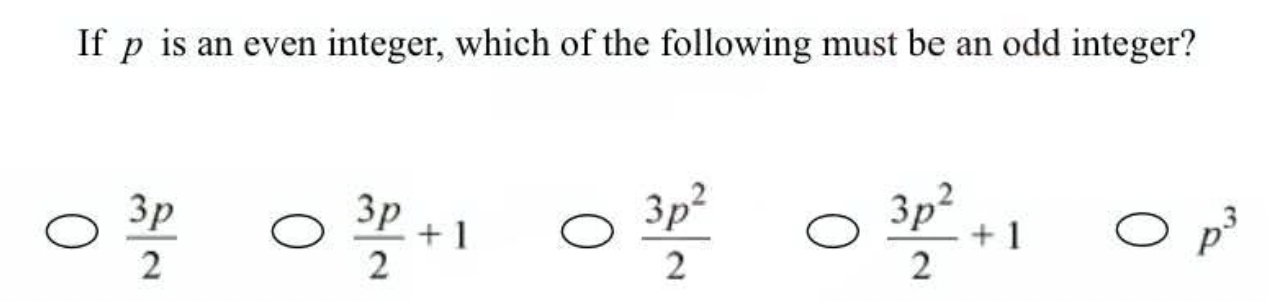
\includegraphics[width=\linewidth]{Even_Odd_Example_Question2.png}
		\caption{2-Sec1-9}
	\end{figure}
	\pause
	$\because p=2k$ \\ 
$\therefore \frac{p}{2}= k$, which is even or odd. \\
$\therefore \frac{p^2}{2}= 2k^2$, which is even. \\
\pause
\bigskip
Answer \textbf{D} 请把5个选项大小排序
\end{frame}

%------------------------------------------------

\subsection{Divisor and the Greatest Common Divisor}
%------------------------------------------------

\begin{frame}
	\frametitle{Definitions \& Examples For A Divisor(Factor)}
	\framesubtitle{约数(因数)}
	\begin{definition}
		When integers are multiplied, each of the multiplied integers is called a
\alert{factor or divisor} of the resulting product
	\end{definition}
	
	\smallskip % Vertical whitespace
	
	\begin{example}
		\begin{itemize}
			\item (2)(3)(10) = 60, so 2,3, and 10 are factors of 60. 
			\item The integers 4, 15, 5, and 12 are also factors of 60. 
			\item \alert{(-2)(-30) = 60}. The negatives of the positive factors are also factors of 60.
			\item 0 is \alert{not} a factor of any integer except \alert{0}.
		\end{itemize}
	\end{example}
	
	\begin{corollary}
		Every integer a is divisible by the trivial divisors, 1 and a. 
	\end{corollary}
\end{frame}

%------------------------------------------------

\begin{frame}
	\frametitle{Definitions \& Examples For The Greatest Common Divisors}
	\framesubtitle{gcd(最大公因数)}
	
	\begin{definition}
	The greatest common divisor (or greatest common factor) of two
nonzero integers c and d is the greatest \alert{positive} integer that is a divisor of
both c and d.
	\end{definition}
	
	\smallskip % Vertical whitespace
	
	\begin{example}
	The least common multiple of 30 and 75 is 150.
		\begin{itemize}
			\item The positive divisors of 30 are 1, 2, 3, 5, 6, 10, 15, and 30.
			\item The positive divisors of 75 are 1, 3, 5, 15, 25, and 75.
			\item The common positive divisors of 30 and 75 are 1, 3, 5, and 15.
			\item The greatest of these is 15.
		\end{itemize}
	\end{example}
\end{frame}

%------------------------------------------------

\begin{frame}
	\frametitle{The Big Question}
	\bigskip
	{\LARGE Is there a better way to find the gcd of two nonzero integers c and d?}
	\bigskip
\end{frame}

%------------------------------------------------
\subsection{Prime v.s. Composite}
\begin{frame}
	\frametitle{Prime V.s. Composite}
	\framesubtitle{质数 V.s. 合数}
	\begin{columns}[t]
	\begin{column}{0.45\textwidth}
	\begin{definition}
		  A \alert{prime number} is an integer \alert{greater than 1} that has only two positive divisors: 1 and itself.
	  \end{definition}

	  \begin{definition}
		  An integer \alert{greater than 1} that is \alert{not} a prime number is called a \alert{composite} number.
	  \end{definition}
	\end{column}
	\begin{column}{0.5\textwidth}
	  	\begin{figure}
		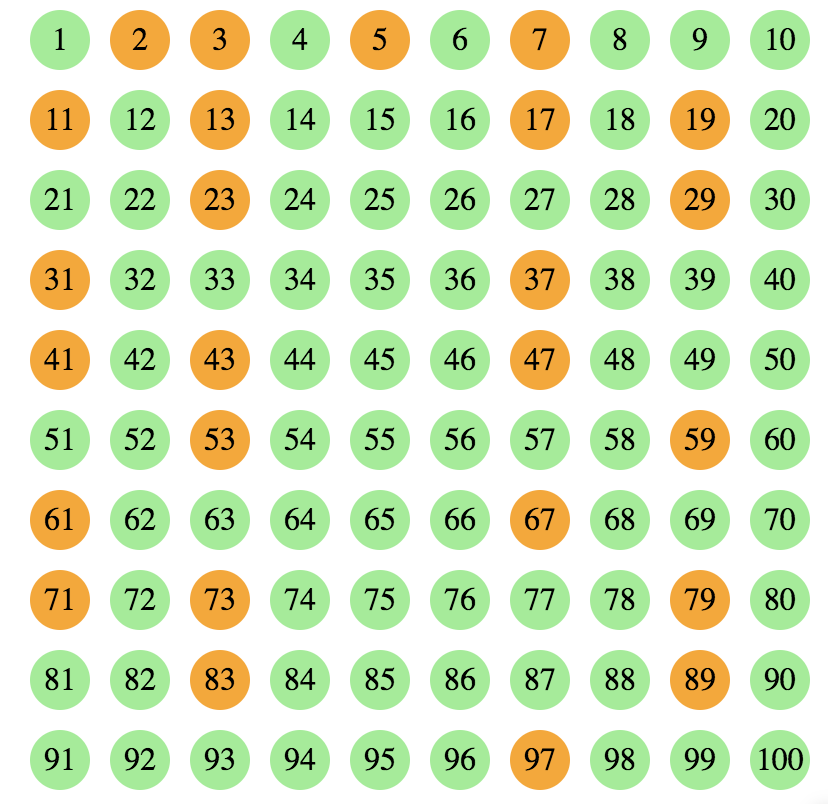
\includegraphics[width=0.8\textwidth]{Prime_Numbers.png}
		\caption{There are 25 prime numbers which are less than 100.}
	\end{figure}
	\end{column}
	\end{columns}


\end{frame}

%------------------------------------------------

\begin{frame}
	\frametitle{Divisible Rules}
	
	\begin{theorem}[Divisible by 2]
		The last digit is even (0, 2, 4, 6, or 8). Thus, Any even number who is greater than 2 is not a prime.
	\end{theorem}
	
	\begin{theorem}[Divisible by 3]
		The Sum of digits if  divisible by 3. For example, 12, 36, 93, 102.
	\end{theorem}

	\begin{theorem}[Divisible by 5]
		The last digit is 0 or 5.
	\end{theorem}
\end{frame}

%------------------------------------------------

\begin{frame}
	\frametitle{Prime Factorization}
	\framesubtitle{质数分解}
	
	\begin{theorem}[Prime Factorization]
		Every integer greater than 1 either is a prime number or can be \alert{uniquely} expressed as a product of factors that are prime numbers, or prime divisors
	\end{theorem}
	
	\smallskip % Vertical whitespace
	
		\begin{columns}[c] % The "c" option specifies centered vertical alignment while the "t" option is used for top vertical alignment
		\begin{column}{0.45\textwidth} % Left column width
				\begin{example}
		\begin{itemize}
			\item $12 = 2^2 \cdot 3$
			\item $81 = 3^3$
			\item $3398 = \pause 2 \cdot 13^2$
			\item $1155 = \pause 3\cdot 5 \cdot 7 \cdot 11$
		\end{itemize}
	\end{example}
		\end{column}
		\begin{column}{0.5\textwidth} % Right column width
		\textbf{First Try!}\\
		 If y is the smallest positive integer such that 3150 multiplied by y is the
square of an integer, then y must be? \\
\smallskip
\pause
$3150= 2 \cdot 3^2 \cdot 5^2 \cdot 7$
\pause
$y \cdot 2 \cdot 3^2 \cdot 5^2 \cdot 7  = x^2$, in which x and y are positive integers.\\
The smallest y $= 2 \cdot 7 = \textbf{14}$\\
		\end{column}
	\end{columns}
\end{frame}

%------------------------------------------------

\begin{frame}
	\frametitle{A Real QR Problem!}
	\framesubtitle{}
	\begin{figure}
		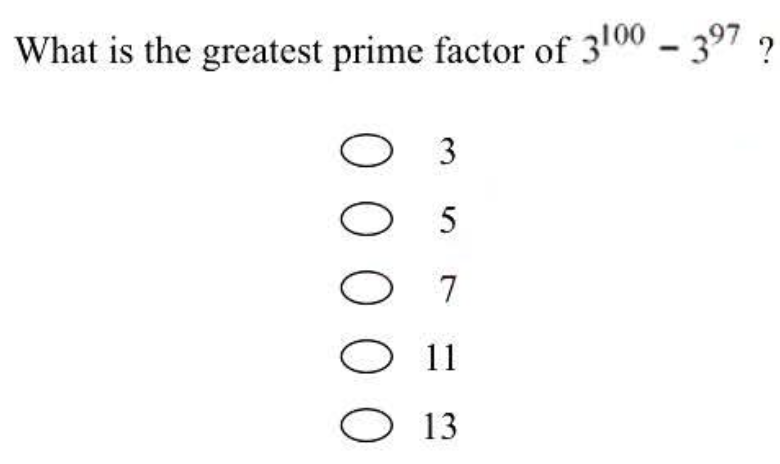
\includegraphics[width=0.5\linewidth]{Prime_Factorization_Example_Question.png}
		\caption{6-Sec3-20}
	\end{figure}
	\pause

		\begin{columns}[t] % The "c" option specifies centered vertical alignment while the "t" option is used for top vertical alignment
		\begin{column}{0.45\textwidth} % Left column width
			\begin{equation*}
			\begin{aligned}
			&3^{100} - 3^{97} \\
			&= 3^{97} \cdot (3^3 - 1) \\
			&= 3^{97} \cdot 26\\&
			= 3^{97} \cdot 2 \cdot 13
			\end{aligned}
	\end{equation*}
		\end{column}
		\begin{column}{0.5\textwidth} % Right column width
		\\ 3 , 2 and 11 are the prime factors. \\
		\pause
		\bigskip
		Answer \textbf{E}
		\end{column}
	\end{columns}
\end{frame}

%------------------------------------------------

\begin{frame}	
	\frametitle{Find GCD with Prime Factorization}
	\framesubtitle{用质数分解找公因数}
		\begin{columns}[t] % The "c" option specifies centered vertical alignment while the "t" option is used for top vertical alignment
			\begin{column}{0.45\textwidth} % Left column width
				What is the gcd of 168 and 96?
			 \begin{enumerate}
			 	\item Prime Factorization of 168: $168=2^3 \cdot 3 \cdot 7$
			 	\item Prime Factorization of 96: $96=2^5 \cdot 3$
			 	\item The gcd equals the products of the common factors with smaller exponent.\\ 取公因子的最小指数 \\ $gcd(168, 96) = 2^3 \cdot 3 = \textbf{24}$
			 	\end{enumerate}

			\end{column}
			\begin{column}{0.5\textwidth} % Right column width
			\begin{figure}
			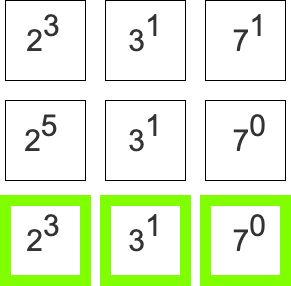
\includegraphics[width=0.8\linewidth]{168_96_GCD.png}
			\caption{The Factors with the smaller exponents}
		\end{figure}
			
			\end{column}
		\end{columns}
\end{frame}

%------------------------------------------------

\begin{frame}
	\frametitle{Have a try!}
	\framesubtitle{先Prime Factorization,然后找Common Factors}
		What is the gcd of 42 and 56?
		 \pause
		 \begin{enumerate}
		 	\item Prime Factorization of 42: $42=3 \cdot 2 \cdot 7$ \pause
		 	\item Prime Factorization of 56: $56=2^3 \cdot 7$ \pause
		 	\item  $gcd(42, 56) = 2 \cdot 7 = \textbf{14}$ 
		 	\end{enumerate}
\end{frame}

%------------------------------------------------


\begin{frame}
	\frametitle{A Real QR Problem!}
	\framesubtitle{}
	\begin{figure}
		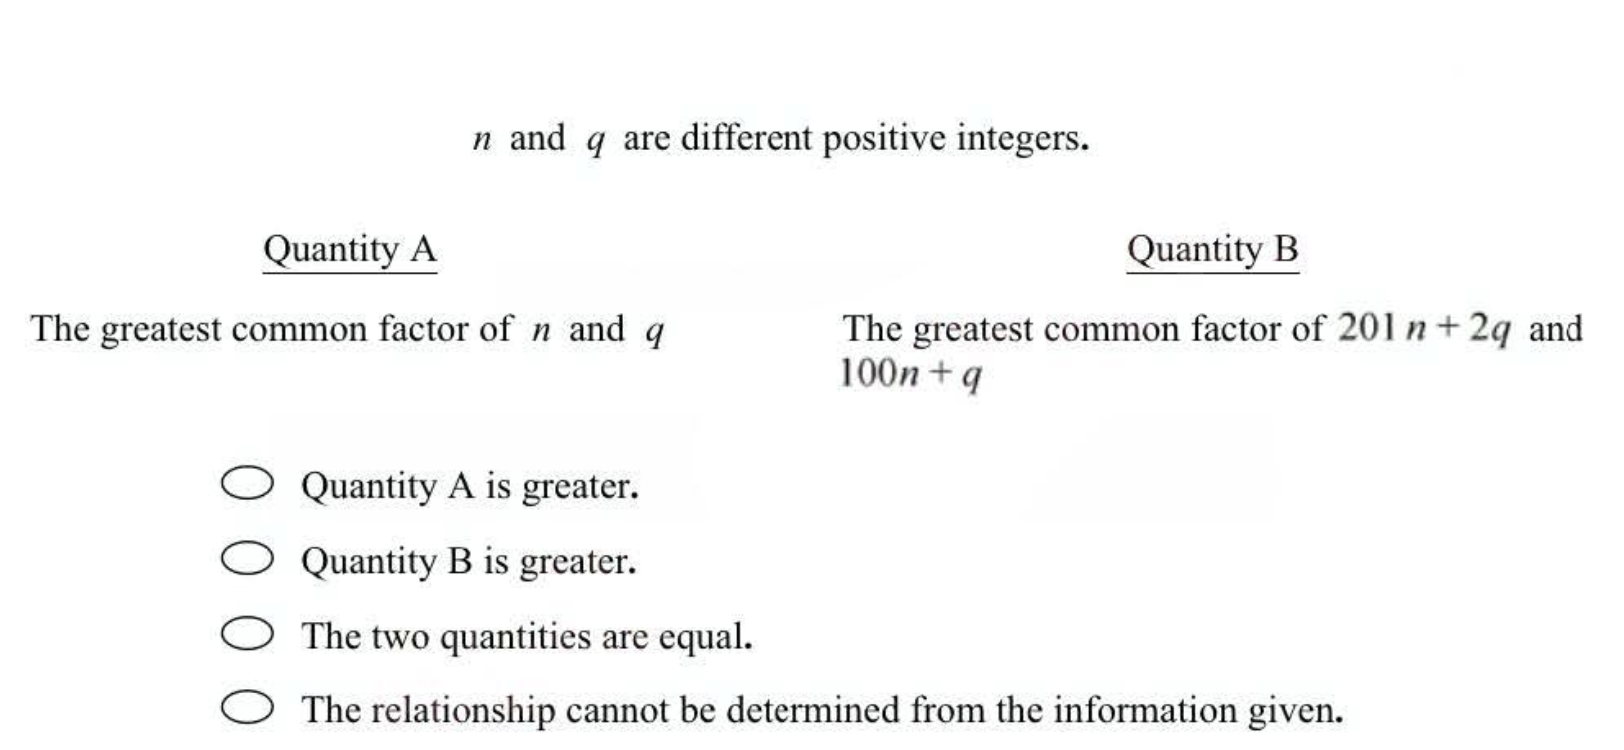
\includegraphics[width=\linewidth]{GCD_Example_Question.png}
		\caption{7-Sec2-7}
	\end{figure}
\bigskip

\end{frame}

%------------------------------------------------


\begin{frame}
	\frametitle{Answer}



  	\begin{columns}[t] % The "c" option specifies centered vertical alignment while the "t" option is used for top vertical alignment
		\begin{column}{0.5\textwidth} % Left column width
			$A = gcd(n, q)$ \\
	$\therefore n = k_1 \cdot gcd(n, q)$ and $q = k_2 \cdot gcd(n, q)$\\
	\bigskip
	\begin{equation*}
		B = gcd(201n + 2q, 100n + q) 
	\end{equation*}
  
				
				\begin{equation*}
				  	\begin{aligned}
				  	&201n + 2q \\&= 67 \cdot 3 n + 2q \\&= gcd(n, q) ( 67 \cdot 3 k_1 + 2k_2)
				  	\end{aligned}
				  \end{equation*}

				  					\begin{equation*}
			  	\begin{aligned}
			  	&100n + q \\&= 2^2\cdot5^2n + q \\&= gcd(n, q) ( 2^2\cdot5^2k_1 + k_2)
			  	\end{aligned}
			  \end{equation*}

		\end{column}
		\begin{column}{0.5\textwidth} % Right column width	
\begin{equation*}
			  	\begin{aligned}
			  	&B = gcd(201n + 2q, 100n + q)\\&=gcd(n,q) \cdot \\ &gcd(67 \cdot 3 k_1 + 2k_2, 2^2\cdot5^2k_1 + k_2)
			  	\end{aligned}
			  \end{equation*}
\pause				
\alert{What if $67 \cdot 3 k_1 + 2k_2$ and $2^2\cdot5^2k_1 + k_2$ are different primes?}\\

	$\because gcd(67 \cdot 3 k_1 + 2k_2, 2^2\cdot5^2k_1 + k_2) \geq 1$  \\ 
	$\therefore  B \geq A $ \\
		\bigskip

\pause
Answer \textbf{D: } The relationship cannot be determined from the information given.
		\end{column}
	\end{columns}
  
	



\end{frame}

%------------------------------------------------

\begin{frame}
	\frametitle{Have Another Try!}
	\framesubtitle{}
	$A = gcd(n, q)$ \\
	
	\bigskip
  $B = gcd(201n + 3q, 96n + 81q)$ \\
\bigskip
\pause
$B \geq 3 \cdot gcd(n, q) > A$\\
Answer \textbf{B: } Quantity B is greater
\end{frame}

%------------------------------------------------

\subsection{Multiple and Least Common Multiple}

%------------------------------------------------

\begin{frame}
	\frametitle{Definitions \& Examples For A Multiple}
	\framesubtitle{倍数}
	\begin{definition}
		We say that an integer is a multiple of each of its factors and that an integer is
divisible by each of its divisors.
	\end{definition}
	
	\smallskip % Vertical whitespace
	
	\begin{example}
		\begin{itemize}
			\item 25 is a multiple of only six integers: 1, 5, 25, and their \alert{negatives}.
			\item The list of positive multiples of 25 has no end: 25, 50, 75, 100, …; likewise, every nonzero integer has infinitely many multiples.
			\item 1 is \alert{not} a multiple of any integer except 1 and −1.
			\item 0 is a multiple of every integer.
		\end{itemize}
	\end{example}
	
\end{frame}

%------------------------------------------------


\begin{frame}
	\frametitle{A Real QR Problem!}
	\framesubtitle{}
	\begin{figure}
		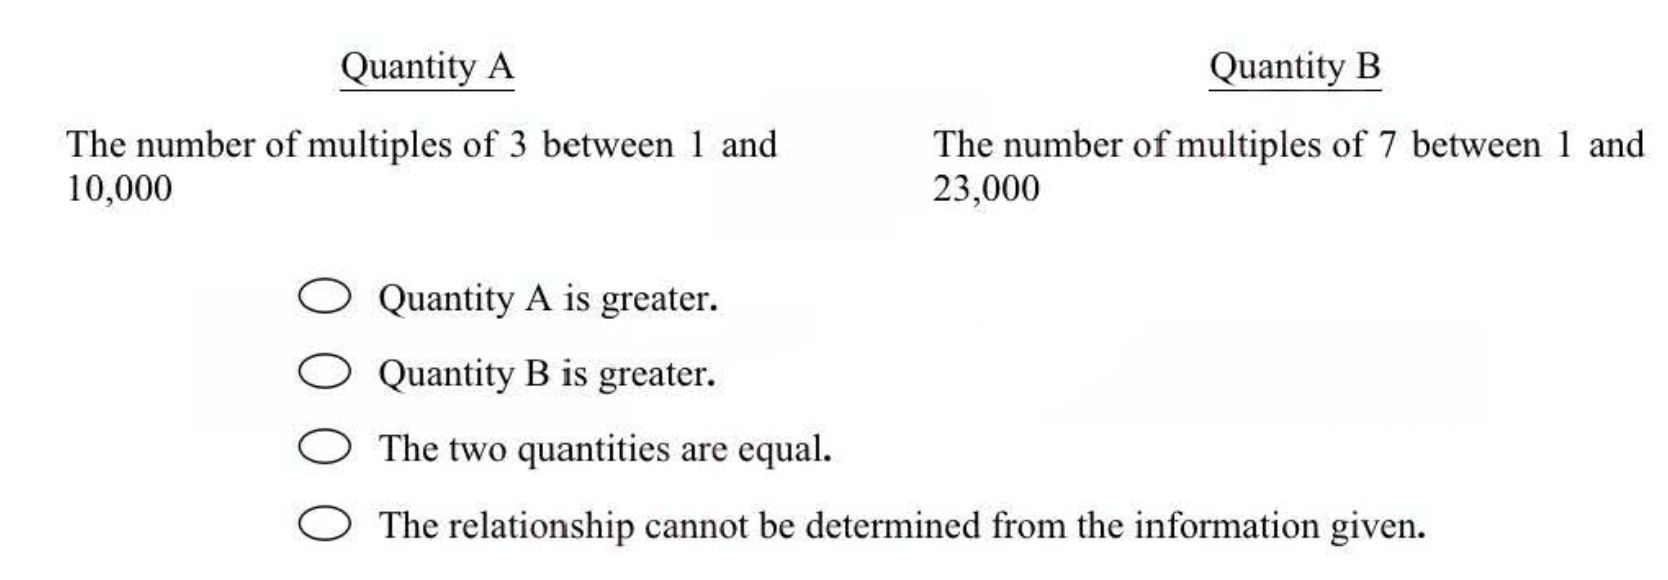
\includegraphics[width=\linewidth]{Multiple_Example_Question1.png}
		\caption{2-Sec1-1}
	\end{figure}
	\pause
x: Multiples of 3 between 1 and 10, 000 \\ $x = 3k_1$, where $k_1 = 1, 2, ..... 333$ \\$x_{max} = 9,999$\\ A = 333 \quad
$333 \cdot 7 = 2,331 > 2300 $ \\
\pause

Answer \textbf{A}
\end{frame}

%------------------------------------------------

\begin{frame}
	\frametitle{Definitions \& Examples For The Least Common Multiple}
	\framesubtitle{lcm(最小公倍数)}
	
	\begin{definition}
	The least common multiple of two nonzero integers c and d is the least \alert{positive} integer that is a multiple of both c and d.
	\end{definition}
	
	\smallskip % Vertical whitespace
	
	\begin{example}
	The least common multiple of 30 and 75 is 150.
		\begin{itemize}
			\item the positive multiples of 30: 30, 60, 90, 120, 150, 180, 210, 240, 270, 300, 330, 390, 420, 450, .....
			\item the positive multiples of 75: 75, 150, 225, 300, 375, 450, .....
			\item The common positive divisors of 30 and 75 are 1, 3, 5, and 15.
			\item The common positive multiples of 30 and 75: 150, 300, 450, .....
		\end{itemize}
	\end{example}
\end{frame}

%------------------------------------------------

\begin{frame}
	\frametitle{The Big Question}
	\bigskip
	{\LARGE How can find the lcm of two nonzero integers?}\\
	\bigskip
	\pause
	{\LARGE \alert{\textbf{Find the gcd!}}}
\end{frame}

%------------------------------------------------


\begin{frame}
	\frametitle{gcd v.s. lcm}
	\framesubtitle{最大公因数 v.s. 最小公倍数}

	
	\begin{columns}[c] % The "c" option specifies centered vertical alignment while the "t" option is used for top vertical alignment
		\begin{column}{0.6\textwidth} % Left column width

				\begin{equation*}
					\begin{split}
						&lcm(c, d) = \frac{\mid c \cdot d \mid}{gcd(c, d)} \\
						\bigskip
				    &\mid c \mid= k_1 \cdot gcd(c, d) \\
				    \bigskip
				    &\mid d \mid= k_2 \cdot gcd(c, d) \\
				    \bigskip
				    &lcm(c, d) = \frac{\mid c \cdot d \mid}{gcd(c, d)} \\
				              &= \frac{[k_1 \cdot gcd(c, d)] \cdot [k_2 \cdot gcd(c, d)] }{gcd(c, d)} \\
				              &= k_1 \cdot gcd(c, d) \cdot k_2
					\end{split}
				\end{equation*}

		\end{column}
		\begin{column}{0.4\textwidth} % Right column width
			\begin{figure}
				\includegraphics[width=\textwidth]{LCM.png}
			\end{figure}
		
		\end{column}
	\end{columns}
\end{frame}


\begin{frame}
	\frametitle{The Big Question}
	\bigskip
	{\LARGE What is the lcm of -12 and 5?  }
	\bigskip
	\pause

	\begin{equation*}
		lcm(c, d) = \frac{\alert{\mid} c \cdot d \alert{\mid}}{gcd(c, d)}
	\end{equation*}

	\begin{alertblock}{How to find the lcm or the gcd of a negative integer and a positive integer}
	    Ignore the negative signs of c and d when it comes to the lcm or the gcd! \\ The lcm and the gcd are both positive!
	\end{alertblock}

\end{frame}



\begin{frame}	
	\frametitle{Find LCM with Prime Factorization}
	\framesubtitle{用质数分解找公倍数}
	\begin{columns}[t] % The "c" option specifies centered vertical alignment while the "t" option is used for top vertical alignment
			\begin{column}{0.45\textwidth} % Left column width
				What is the lcm of 168 and 96?
			 \begin{enumerate}
			 	\item Prime Factorization of 168: $168=2^3 \cdot 3 \cdot 7$
			 	\item Prime Factorization of 96: $96=2^5 \cdot 3$
			 	\item The lcm equals the products of all factors with larger exponent.\\ 取所有因子的最大指数 \\ $lcm(168, 96) = 2^5 \cdot 3 \cdot 7= \textbf{672}$
			 	\end{enumerate}
			\end{column}

			\begin{column}{0.5\textwidth} % Right column width
			  \begin{figure}
			    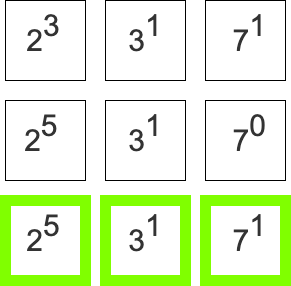
\includegraphics[width=0.8\linewidth]{168_96_LCM.png}
			    \caption{The Factors with the larger exponents}
		    \end{figure}
			\end{column}
	\end{columns}
\end{frame}

%------------------------------------------------

\begin{frame}
	\frametitle{Have a try!}
	\framesubtitle{先Prime Factorization,然后找 Factors with larger exponents}
		What is the lcm of 24 and 78?
		 \pause
		 \begin{enumerate}
		 	\item Prime Factorization of 24: $24=2^3 \cdot 3$ \pause
		 	\item Prime Factorization of 78: $56=2 \cdot 3 \cdot 13$ \pause
		 	\item  $lcm(24, 78) = 2^3 \cdot 3 \cdot 13 = \textbf{312}$ 
		 	\end{enumerate}
\end{frame}

%------------------------------------------------

\begin{frame}
	\frametitle{Have a try!}
	\framesubtitle{}
		If M is the least common multiple of 90, 196, and 300, which of the following is NOT a factor of M?
		 \begin{enumerate}[A]
		 	\item 600
		 	\item 700
		 	\item  900
		 	\item 2100
		 	\item 4900
		 	\end{enumerate}

		 	\pause 


	\begin{columns}[t] % The "c" option specifies centered vertical alignment while the "t" option is used for top vertical alignment
		\begin{column}{0.45\textwidth} % Left column width
						\begin{equation*}
					\begin{split}
					&90 = 2 \cdot 3^2 \cdot 5 \\
			 		&196 = 2^2 \cdot 7^2 \\
			 		&300 =  2^2 \cdot 3 \cdot 5^2 \\
			 		&lcm(90, 196, 300) \\ &= 2^2 \cdot 3^2 \cdot 5^2\cdot 7^2   
					\end{split}
				\end{equation*}

		\end{column}
		\begin{column}{0.5\textwidth} % Right column width
						\begin{enumerate}[A]
		 	\item $600 = \alert{2^3} \cdot 3 \cdot 5^2$
		 	\item $700 = 2^2 \cdot 5^2 \cdot 7 $
		 	\item  $900 = 2^2 \cdot 3^2 \cdot 5^2$
		 	\item $2100 = 2^2 \cdot 3 \cdot  5^2  \cdot 7$
		 	\item $4900 = 2^2 \cdot 5^2 \cdot 7^2$
		 	\end{enumerate} 
		 	Answer \textbf{A}
		\end{column}
	\end{columns}
\end{frame}

%------------------------------------------------

%------------------------------------------------
% question; ignore the sign; lcm demo;have a try; have a try mayu; real QR question

%------------------------------------------------


%------------------------------------------------
\subsection{Quotient and Remainder}
%------------------------------------------------

\begin{frame}
	\frametitle{Definitions \& Examples For The Quotient and Remainder}
	\framesubtitle{商数和余数}
	
	\begin{definition}
	For any integer a and any \alert{positive} integer n, there exist unique integers q and r such that \alert{$0\leq r < n$} and $a = qn + r$. \\
	The value q is the quotient of the division. \\ The value r is the remainder
	\end{definition}
	
	\smallskip % Vertical whitespace
	
	\begin{example}
		\begin{itemize}
			\item $100 \div 45 = 2 \cdots 10 $
			\item $24 \div 2 = 12 \cdots 0 $ 
			\item $ (-32 \div 3 = -11 \cdots 1 $ 
		\end{itemize}
	\end{example}
\end{frame}

%------------------------------------------------


\begin{frame}
	\frametitle{The Loop Of Remainders: Modular Arithmetic}
	\framesubtitle{余数的循环}
	\textbf{Modulus 7}

		\begin{columns}[t] % The "c" option specifies centered vertical alignment while the "t" option is used for top vertical alignment
		\begin{column}{0.3\textwidth} % Left column width
		$-7 \mod 7 = 0$ \\
		$-1 \mod 7 = 6$ \\
		$-2 \mod 7 = 5$ \\
		$-3 \mod 7 = 4$ \\
		$-4 \mod 7 = 3$ \\
		$-5 \mod 7 = 2$ \\
		$-6 \mod 7 = 1$ \\
		\end{column}
		\begin{column}{0.3\textwidth} % Right column width
		$0 \mod 7 = 0$ \\
		$1 \mod 7 = 1$ \\
		$2 \mod 7 = 2$ \\
		$3 \mod 7 = 3$ \\
		$4 \mod 7 = 4$ \\
		$5 \mod 7 = 5$ \\
		$6 \mod 7 = 6$ \\
		\end{column}

		\begin{column}{0.3\textwidth} % Right column width
		$7 \mod 7 = 0$ \\
		$8 \mod 7 = 1$ \\
		$9 \mod 7 = 2$ \\
		$10 \mod 7 = 3$ \\
		$11 \mod 7 = 4$ \\
		$12 \mod 7 = 5$ \\
		$13 \mod 7 = 6$ \\
		\end{column}
	\end{columns}
\end{frame}

%------------------------------------------------


\begin{frame}
	\frametitle{A Real QR Problem!}
	\framesubtitle{}
	\begin{figure}
		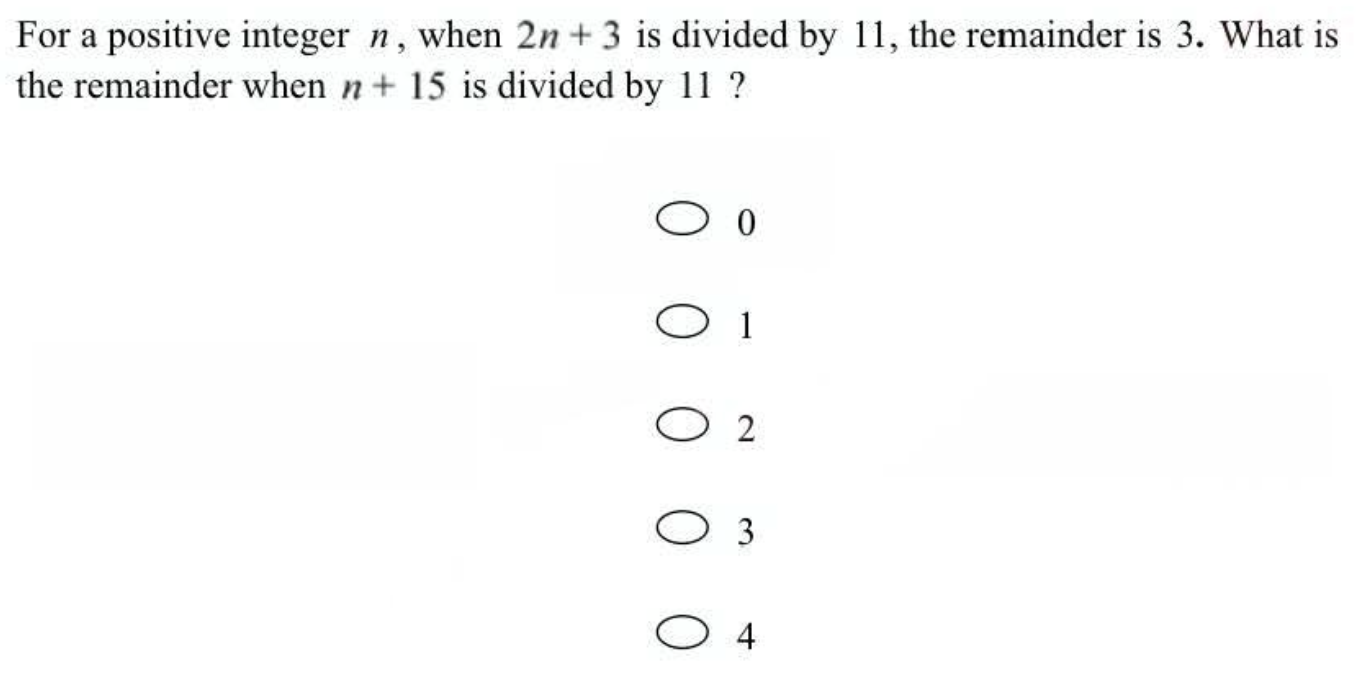
\includegraphics[width=\linewidth]{Remainder_Example_Question1.png}
		\caption{1-Sec2-20}
	\end{figure}

\end{frame}

%------------------------------------------------

\begin{frame}
	\frametitle{Answer}
	\framesubtitle{}

	$\because (2n + 3) \mod 11 = 3$ \\
	$\therefore 2n  \mod 11 = 0$ \\
	$\therefore n  \mod 11 = 0$ \\
	$\therefore (n + 15) \mod 11 = 15 \mod 11 = 4$ \\
\pause
\bigskip
Answer \textbf{E: } $ (n + 15) \mod 11 = 4$
\end{frame}

%------------------------------------------------

\begin{frame}
	\frametitle{A Real QR Problem!}
	\framesubtitle{}
	\begin{figure}
		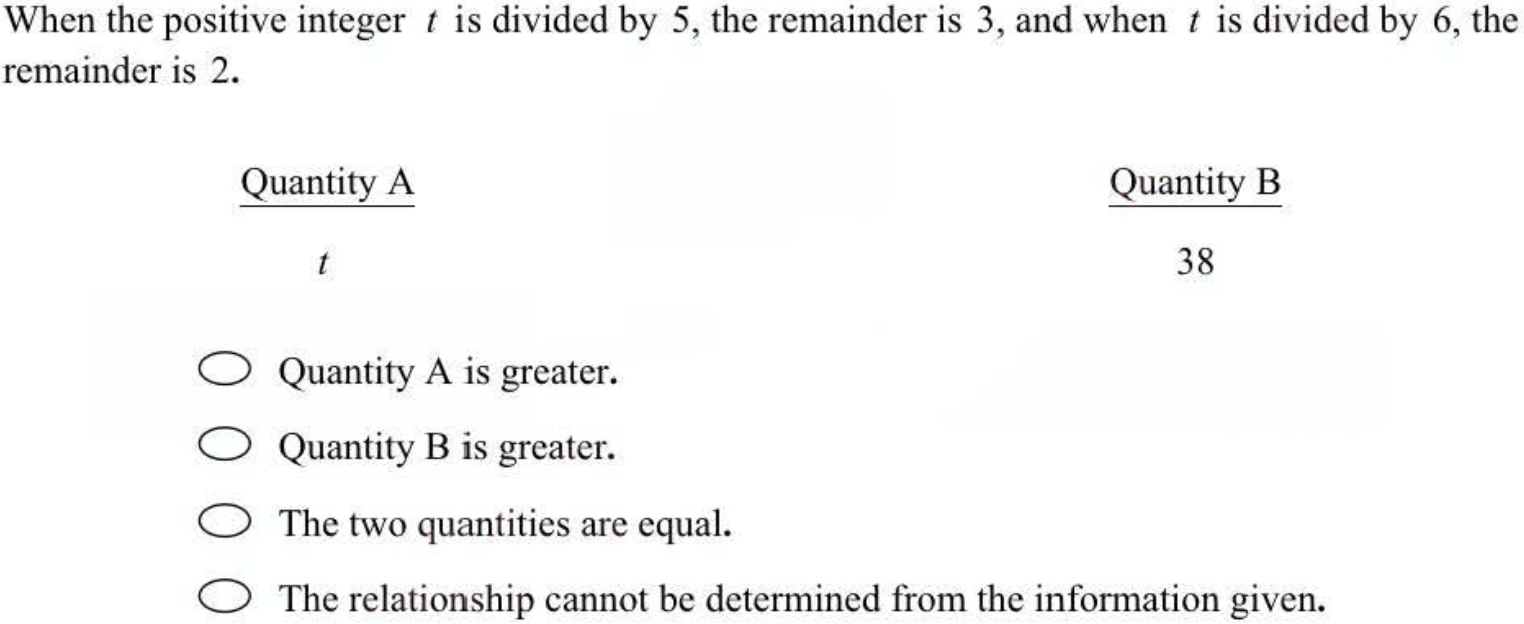
\includegraphics[width=\linewidth]{Remainder_Example_Question2.png}
		\caption{3-Sec2-6}
		\end{figure}
\end{frame}

%------------------------------------------------

\begin{frame}
	\frametitle{Answer}
	\framesubtitle{}

	$\because t \mod 5 = 3 \therefore t = 5  k_1 + 3$ \\
	$\because t \mod 6 = 2 \therefore t = 6  k_2 + 2$ \\
	$\therefore 6 k_2 + 2  = 5  k_1 + 3 $ \\
	$\therefore k_2 = \frac{5  k_1 + 1}{6}$ \\

	\bigskip
	$\therefore (5k_1 + 1)$ is a multiple of 6. 
		\begin{table}
		\begin{tabular}{l l l l}
			\toprule
			\textbf{$5  k_1 + 1$} & \textbf{$k_1$} & \textbf{$k_2$} & \textbf{t}\\
			\midrule
			6& 1 & 1 & 8 \\
			36& 7 & 6 & \alert{38} 答案已确定\\
			66& 13 & 11 & 68 \\
			\bottomrule
		\end{tabular}
		\caption{Several Possible values for $k_1, k_2$ and t}
	\end{table}

	

\bigskip
Answer \textbf{D: } The relationship cannot be determined from the information given.
\end{frame}

%------------------------------------------------



\begin{frame}
	\frametitle{A Real QR Problem!}
	\framesubtitle{注意 “NOT Possible”}
	\begin{figure}
		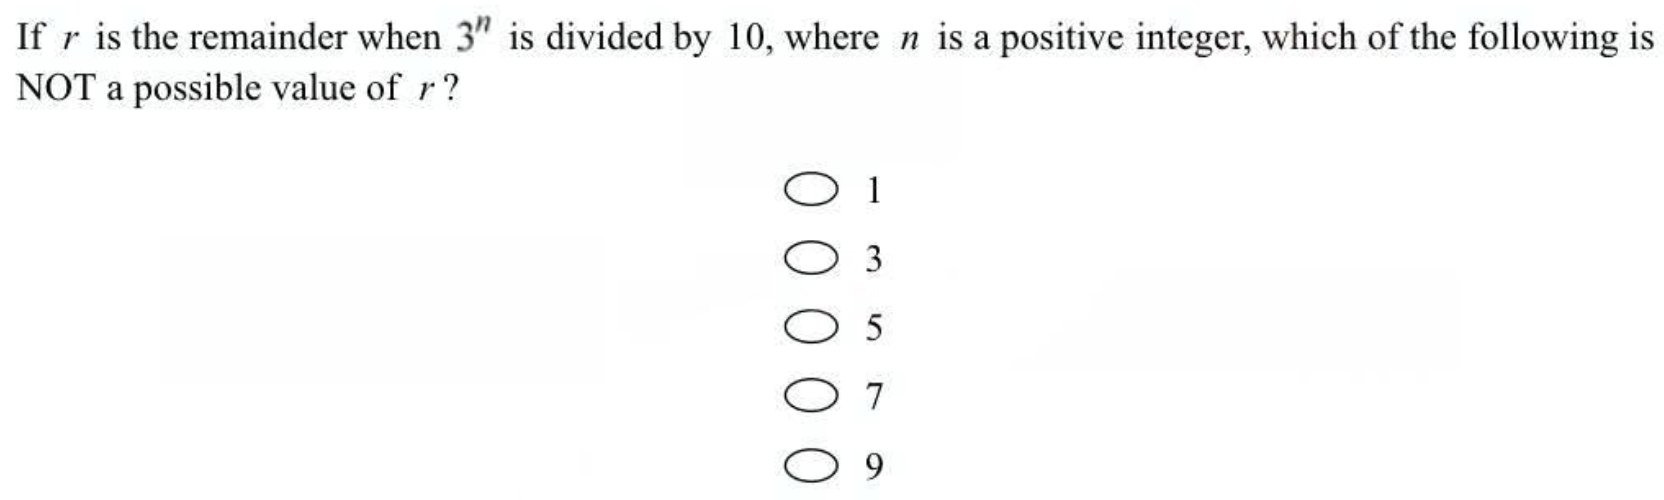
\includegraphics[width=\linewidth]{Remainder_Example_Question3.png}
		\caption{4-Sec1-11}
		\end{figure}
\end{frame}

%------------------------------------------------


\begin{frame}
	\frametitle{Answer}
	\framesubtitle{看个位}

		\begin{table}
		\begin{tabular}{l l l}
			\toprule
			\textbf{$n$} & \textbf{$3^n$} & \textbf{$r = 3^n \mod 10$} \\
			\midrule
			1& 3 & 3  \alert{B}\\
			2& 9 & 9 \alert{E}\\
			3& 27 & 7 \alert{D}\\
			4& 81 & 1 \alert{A}\\
			5& 243 & 3 \alert{B}\\
			\vdots &\vdots & \vdots\\
			\bottomrule
		\end{tabular}
		% \caption{Several Possible values for n, $3^n$, and $r = 3^n \mod 10$.}
	\end{table}

	

\bigskip
Answer \textbf{C: } 5 is Not a possible values for r. \\
What if $r=7^n$?
\end{frame}

%------------------------------------------------
%----------------------------------------------------------------------------------------
%	CLOSING SLIDE
%----------------------------------------------------------------------------------------

\begin{frame}[plain] % The optional argument 'plain' hides the headline and footline
	\begin{center}
		{\Huge 1 Min Break}
		\bigskip\bigskip % Vertical whitespace
		
		{\LARGE Questions? Comments?}
	\end{center}
\end{frame}

%----------------------------------------------------------------------------------------

\begin{frame}
\frametitle{Initiate The Sonic Mode!}
		\begin{figure}
			
\includegraphics[width=\linewidth]{Sonic.png}
		\end{figure}
\end{frame}

\section{Fractions}


%------------------------------------------------
\begin{frame}
\frametitle{Numerator, Denominator, The Common Denominator and The Mixed Number}
	\begin{block}{Numerator V.s. Denominator \quad 分子 v.s. 分母}
				A fraction is a number of the form where c and d are integers and \alert{$d\neq 0$}. \\
				The integer c is called the numerator of the fraction. \\  
				The integer d is called the denominator.
	\end{block}

	\begin{block}{Common Denominator \quad 公分母}
				The common denominator is a common multiple (ideally the least common multiple) of the denominators of two fractions.\\
				The common denominator of $\frac{1}{3}$ and $\frac{2}{5}$ is 15.
	\end{block}


\end{frame}

%------------------------------------------------
\begin{frame}
\frametitle{ The Mixed Number}

	\begin{block}{Mixed Number \quad 带分数}
	A mixed number consists of an integer part and a fraction part, where the fraction part has a value \alert{between 0 and 1}.\\
	The mixed number $4\frac{3}{8}$ means $4 + \frac{3}{8}$.
	\end{block}
\end{frame}

	
%------------------------------------------------

\begin{frame}
\frametitle{Reciprocal}

	\begin{block}{Reciprocal \quad 倒数}
	The reciprocal of $\frac{c}{d}$ is $\frac{d}{c}$, where both c and d are \alert{non-zero} numbers. 
	\end{block}
\end{frame}

	
%------------------------------------------------
\section{Exponents and Roots}
\subsection{Exponents}

%------------------------------------------------
\begin{frame}
\frametitle{Exponents}
\framesubtitle{指数}

	\begin{columns}[c] % The "c" option specifies centered vertical alignment while the "t" option is used for top vertical alignment
		\begin{column}{0.45\textwidth} % Left column width
				\begin{alertblock}{The Power of Negative Numbers}
						\begin{itemize}
							\item A negative number raised to an even power is always positive.
							\item A negative number raised to an odd power is always negative. 
					\end{itemize}
			 \end{alertblock}
	\begin{exampleblock}{奇负偶正}
		$(-5)^{2n + 1} <0 $, where $n =\ldots, -1, 0 , 1, \ldots$ \\
		$(-5)^{2n } > 0 $, where $n =\ldots, -1, 0 , 1, \ldots$ \\
	\end{exampleblock}

		\end{column}
		\begin{column}{0.5\textwidth} % Right column width
		\begin{figure}
		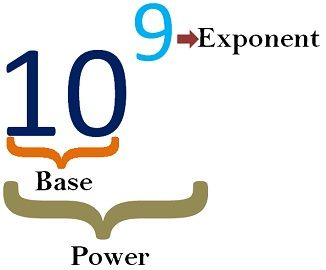
\includegraphics[width=0.5\linewidth]{exponent-vs-power.jpeg}
	\end{figure}
		\end{column}
	\end{columns}
	
\end{frame}
%------------------------------------------------

	\begin{frame}
	\frametitle{Have a try!}
	\framesubtitle{注意到底是指数到底是减还是放在分母里}
	\begin{table}
		\begin{tabular}{l l l}
			\toprule
			$a^m + a^n= \quad $ & $a^m \div a^n = \quad$ & $(a^m)^n = \quad$ \\
      $a^m - a^n= \quad $ & $a^m \cdot b^m = \quad$ & $(a^{m/n} = \quad$ \\
      $a^m \cdot a^n= \quad $ & $a^m \div b^m = \quad$ & $ a^{-r} = \quad$ \\
			\bottomrule
		\end{tabular}
		\caption{Complete the equations}
	\end{table}

	\pause

		\begin{table}
		\begin{tabular}{l l l}
			\toprule
			$a^m + a^n=  a^m(1 + a^{n-m}) $ & $a^m \div a^n = a^{n-m}$ & $(a^m)^n = a^{mn}$ \\
      $a^m - a^n= a^m(1 - a^{n-m}) $ & $a^m \cdot b^m = (ab)^{m}$ & $a^{m/n} = \sqrt[n]{a^m}$ \\
      $a^m \cdot a^n=  a^{m + n}$ & $a^m \div b^m = (\frac{a}{b})^m$ & $ a^{-r} = \frac{1}{a^r}$ \\
			\bottomrule
		\end{tabular}
		\caption{Complete the equations}
	\end{table}

\end{frame}
%------------------------------------------------

\subsection{Roots}
\begin{frame}
\frametitle{Roots}
\framesubtitle{开根号}

	\begin{columns}[c] % The "c" option specifies centered vertical alignment while the "t" option is used for top vertical alignment

		\begin{column}{0.3\textwidth} % Right column width
		\begin{equation*}
			\sqrt[n]{a} = a^{\frac{1}{n}}
		\end{equation*}
		\bigskip
		\begin{equation*}
			(\sqrt[n]{a})^n = a
		\end{equation*}
		\end{column}

				\begin{column}{0.7\textwidth} % Left column width
					\begin{alertblock}{Odd Roots V.s. Even Roots}
					\begin{itemize}
							\item A negative number raised to an even power is always positive.
							\item A negative number raised to an odd power is always negative. 
					\end{itemize}
					For odd order roots, there is exactly one root for every number n, even when n is negative. \\
					For even order roots, there are exactly one positive and one negative roots for every positive number n and \alert{no roots for any negative number n}.
				 \end{alertblock}

					\begin{exampleblock}{开偶次方两个根}
						One Cube roots for 64: $\sqrt[3]{64} = 4$ \\
						Two Fourth roots for 64: $\pm \sqrt[2]{64} = \pm 8$
					\end{exampleblock}

		\end{column}
	\end{columns}
	
\end{frame}
%------------------------------------------------

\begin{frame}
	\frametitle{Have a try!}
	\framesubtitle{}
	The function f(x) is defined for each positive three-digit integer n by $f(n) = 2^x3^y5^z$,
where x, y, and z are hundreds, tens, and units digits of n, respectively. If m and v are
three-digit positive integers such that f(m) = 9f(v), then what is the value of m – v? \\
\bigskip
\pause
$m=100x_1 + 10y_1 + z_1$ and $v = 100x_2 + 10y_2 + z_2$\\
$\because f(m) = 9f(v) \quad \therefore 2^{x_1}3^{y_1}5^{z_1} = 9\cdot2^{x_2}3^{y_2}5^{z_2}$\\
$\therefore 2^{x_1}3^{y_1}5^{z_1} = 2^{x_2}3^{y_2 +2}5^{z_2}$ \\
\smallskip
By the uniqueness of Prime Factorization,\\
$x_1 = x_2, \quad y_1 = y_2 + 2,  \quad z_1 = z_2$\\
$m - v = (100x_1 + 10y_1 + z_1) - (100x_2 + 10y_2 + z_2) = 10(y_1 -y_2) = 20$\\

\bigskip
Answer \textbf{20}
\end{frame}

%------------------------------------------------


\begin{frame}
	\frametitle{Have a try!}
	\framesubtitle{}

		\begin{columns}[t] % The "c" option specifies centered vertical alignment while the "t" option is used for top vertical alignment
		\begin{column}{0.45\textwidth} % Left column width
					Which of the following inequalities has a solution set that, when graphed in the
			number line, is a single line segment of finite length?\\
			   \begin{enumerate}[A]
			   \item $x^4 \geq 16$
			   \item $x^3 \leq 27$
			   \item $x^2 \geq 16$
			   \item $2 \leq \mid x \mid \leq 5$
			   \item $2 \leq 3x + 4 \leq 6$
			   \end{enumerate}
		\end{column}
		\begin{column}{0.5\textwidth} % Right column width
				\pause
				\begin{enumerate}[A]
			   \item $x^4 \geq 16 $ has two roots but is with infinite length
			   \item $x^3 \leq 27$ has  one roots but is with infinite length
			   \item $x^2 \geq 16$ has  two roots but is with infinite length
			   \item $2 \leq \mid x \mid \leq 5$ two segments of finite length
			   \item $2 \leq 3x + 4 \leq 6$ a single segment of finite length
			   \end{enumerate}
				\bigskip
				Answer \textbf{E}
		\end{column}
	\end{columns}
\end{frame}

%------------------------------------------------

\section{Decimal}
%-----------------------------------------------

\subsection{Terminating and  Repeating Decimal}

%------------------------------------------------

\begin{frame}
\frametitle{Terminating and  Repeating Decimal}
\framesubtitle{终止小数 循环小数}

		\begin{figure}
		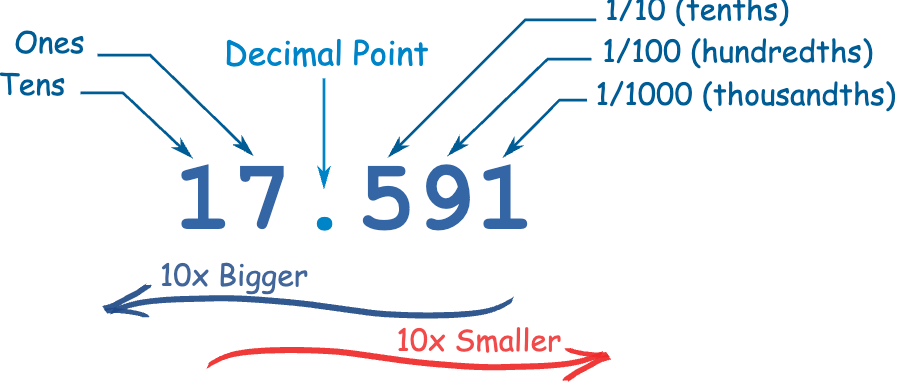
\includegraphics[width=0.5\linewidth]{Decimal.png}
	  \end{figure}

	  \begin{columns}[t] % The "c" option specifies centered vertical alignment while the "t" option is used for top vertical alignment
			\begin{column}{0.45\textwidth} % Left column width
						\begin{exampleblock}{Terminating Decimal}
								\begin{itemize}
									\item $\frac{3}{8} = 0.375$
									\item $\frac{259}{40} = 6475$
								\end{itemize}							
						\end{exampleblock}
			\end{column}

			\begin{column}{0.5\textwidth} % Right column width
			\begin{exampleblock}{Repeating Decimal}
								\begin{itemize}
									\item $\frac{25}{12} = 2.08333 \ldots$
									\item $\frac{15}{14} = 1.0\overline{714285}$
								\end{itemize}	
			\end{exampleblock}
			\end{column}
	\end{columns}
\end{frame}

%------------------------------------------------

\begin{frame}
	\frametitle{A Real QR Problem!}
	\framesubtitle{}
	\begin{figure}
		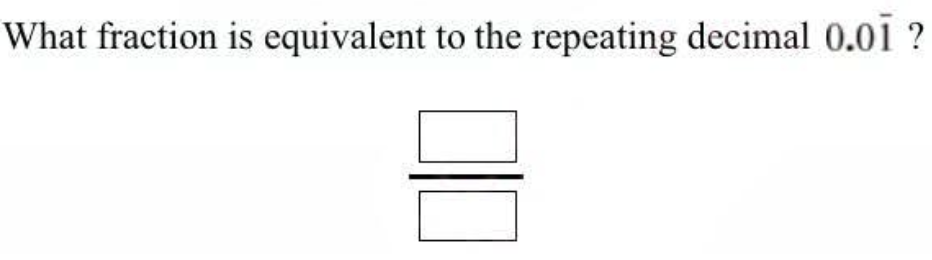
\includegraphics[width=0.6\linewidth]{Decimal_Example_Question1.png}
		\caption{7-Sec2-17}
	\end{figure}
	\pause
\begin{equation*}
	\begin{aligned}
	&0.0\overline{1}  \\
	& =\frac{1}{10} \times 0.\overline{1} \\
	& =\frac{1}{10} \times  \frac{1}{3} \times 0.\overline{3} \\
	& =\frac{1}{10} \times  \frac{1}{3} \times \frac{1}{3} \\
	& = \frac{1}{90}\\
	\end{aligned}
\end{equation*}
\pause
\bigskip
Answer \textbf{$\frac{1}{90}$} \quad what about $0.0\overline{7}$, $0.8\overline{7}$, or $3.1\overline{52}$?
\end{frame}

%------------------------------------------------

\subsection{Rational Numbers v.s. Irrational Numbers}

%------------------------------------------------

\begin{frame}
\frametitle{Rational Numbers v.s. Irrational Numbers}
\framesubtitle{有理数 无理数}

	  \begin{columns}[t] % The "c" option specifies centered vertical alignment while the "t" option is used for top vertical alignment
			\begin{column}{0.45\textwidth} % Left column width
							\begin{theorem}[Rational Numbers]
								Every rational number can be expressed as a terminating or repeating decimal.
							\end{theorem}

						\begin{exampleblock}{Rational Numbers}
								\begin{itemize}
									\item 6.67384 × 10−11
									\item 6.626070040 × 10−34
								\end{itemize}							
						\end{exampleblock}
			\end{column}

			\begin{column}{0.5\textwidth} % Right column width
							\begin{theorem}[Irrational Numbers]
												Every irrational number can be expressed as a non-terminating or non-repeating decimal.
							\end{theorem}
			\begin{exampleblock}{Irrational Numbers}
								\begin{itemize}
									\item $2.718281828459045\ldots$
									\item $\sqrt{2} = 1.41421356237 \ldots$
									\item $3.141592653589793238 \ldots$
								\end{itemize}	
			\end{exampleblock}
			\end{column}
	\end{columns}
\end{frame}

%------------------------------------------------

\section{Ratio}

%------------------------------------------------

\begin{frame}
	\frametitle{Language of the Prompt}
	\framesubtitle{注意题干语言}
	{\LARGE Th ratio $r:s:t$:} 
	\begin{quote}
	{\LARGE r to s to t}
	\end{quote}
\end{frame}

%------------------------------------------------

\begin{frame}
	\frametitle{A Real QR Problem!}
	\framesubtitle{}
	\begin{figure}
		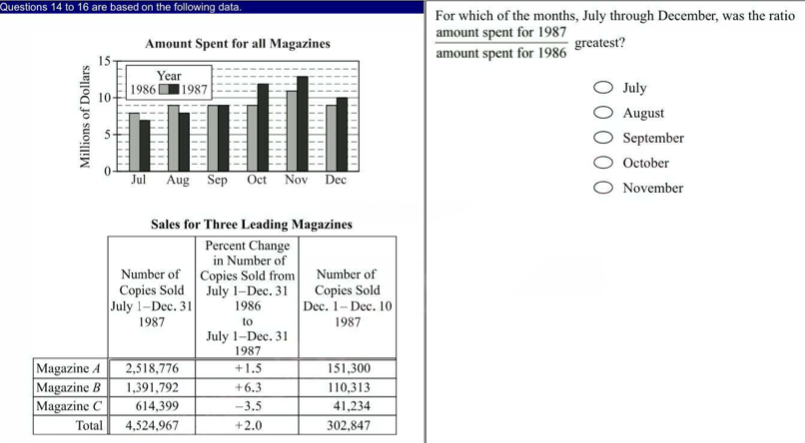
\includegraphics[width=\linewidth]{Ratio_Example_Question1.png}
		\caption{9-Sec1-14}
	\end{figure}

\end{frame}

%------------------------------------------------

\begin{frame}
	\frametitle{Answer}
	\framesubtitle{分子大,分母小,看相差的条相比分母的占比}

	\begin{figure}
		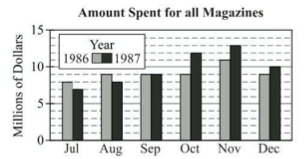
\includegraphics[width=0.5\linewidth]{Ratio_Example_Question1_1.png}
		\caption{9-Sec1-14}
	\end{figure}

For Jul, Aug, Sep, $\frac{amount \ spent \ for 1987}{amount \ spent \ for 1986} \leq 1$; \\
For Oct, Nov, Dec, $\frac{amount \ spent \ for 1987}{amount \ spent \ for 1986} > 1$. \\
Oct have the greatest difference but the least denominator. \\


	

\bigskip
Answer \textbf{D: } October\\
\end{frame}

%------------------------------------------------

\section{Percent}

%------------------------------------------------
\subsection{Whole v.s. Part}

\begin{frame}
	\frametitle{Whole(Base)v.s. Part}
	\frametitle{整理(标准基)v.s. 部分}
	\begin{definition}
		A \alert{prime number} is a number that has exactly two divisors.
	\end{definition}
	
	\smallskip % Vertical whitespace
	
	\begin{example}
		\begin{itemize}
			\item 2 is prime (two divisors: 1 and 2).
			\item 3 is prime (two divisors: 1 and 3).
			\item 4 is not prime (\alert{three} divisors: 1, 2, and 4).
		\end{itemize}
	\end{example}
	
	\smallskip % Vertical whitespace
	
	You can also use the \texttt{theorem}, \texttt{lemma}, \texttt{proof} and \texttt{corollary} environments.
\end{frame}

%------------------------------------------------

\begin{frame}
	\frametitle{Have a try!}
	\framesubtitle{注意 “Nearest Whole Percent”}
	\begin{figure}
		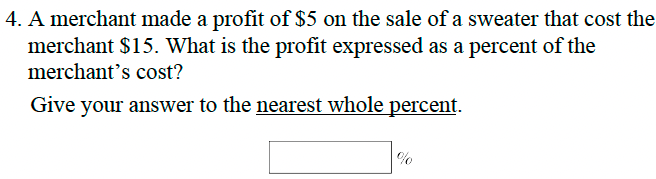
\includegraphics[width=\linewidth]{Percent_Example_Question_2.png}
		\caption{og-p205-4}
	\end{figure}
	\pause
$\frac{5}{15} = 33.\overline{3} \%$ \\

\pause
\bigskip
Answer \textbf{33}
\end{frame}

%------------------------------------------------

\begin{frame}
	\frametitle{A Real QR Problem!}
	\framesubtitle{}
	\begin{figure}
		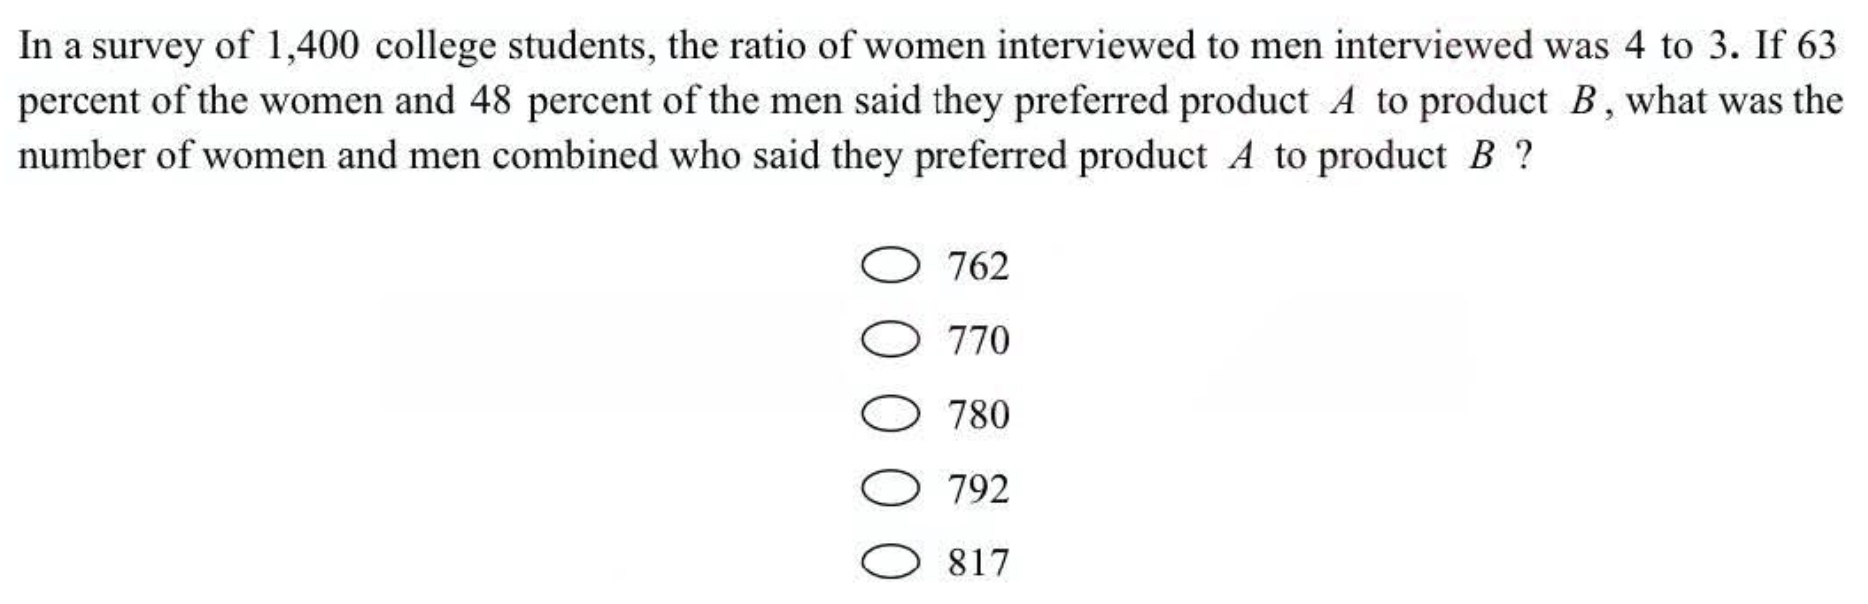
\includegraphics[width=\linewidth]{Percent_Example_Question_1.png}
		\caption{8-Sec1-10}
	\end{figure}
	\pause

\pause
\bigskip
Answer \textbf{D}
\end{frame}

%------------------------------------------------

\subsection{Percent Increase, Percent Decrease, and Percent Change}



% \section{Text Examples} % Sections are added in order to organize your presentation into discrete blocks, all sections and subsections are automatically output to the table of contents as an overview of the talk but NOT output in the presentation as separate slides

% %------------------------------------------------

% \begin{frame}
% 	\frametitle{A Real QR Problem!}
% 	\framesubtitle{}
% 	\begin{figure}
% 		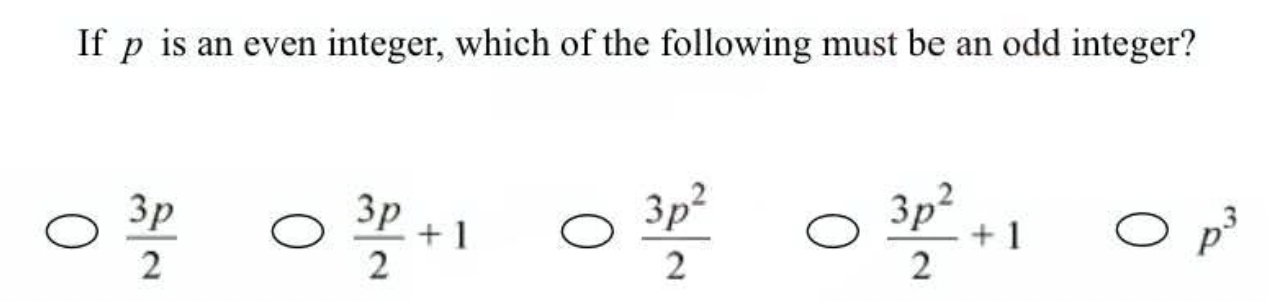
\includegraphics[width=\linewidth]{Even_Odd_Example_Question2.png}
% 		\caption{2-Sec1-9}
% 	\end{figure}
% 	\pause

% \pause
% \bigskip
% Answer \textbf{D}
% \end{frame}

% %------------------------------------------------


% \begin{frame}
% 	\frametitle{Have a try!}
% 	\framesubtitle{}
% \pause
% \bigskip
% Answer \textbf{D}
% \end{frame}

% %------------------------------------------------

% \subsection{Paragraphs and Lists}

% \begin{frame}
% 	\frametitle{Paragraphs of Text}

% 	Sed iaculis \alert{dapibus gravida}. Morbi sed tortor erat, nec interdum arcu. Sed id lorem lectus. Quisque viverra augue id sem ornare non aliquam nibh tristique. Aenean in ligula nisl. Nulla sed tellus ipsum. Donec vestibulum ligula non lorem vulputate fermentum accumsan neque mollis.
	
% 	\bigskip % Vertical whitespace
	
% 	% Quote example
% 	\begin{quote}
% 		Sed diam enim, sagittis nec condimentum sit amet, ullamcorper sit amet libero. Aliquam vel dui orci, a porta odio.\\
% 		--- Someone, somewhere\ldots
% 	\end{quote}
	
% 	\bigskip % Vertical whitespace
	
% 	Nullam id suscipit ipsum. Aenean lobortis commodo sem, ut commodo leo gravida vitae. Pellentesque vehicula ante iaculis arcu pretium rutrum eget sit amet purus. Integer ornare nulla quis neque ultrices lobortis.
% \end{frame}

% %------------------------------------------------

% \begin{frame}
% 	\frametitle{Lists}
% 	\framesubtitle{Bullet Points and Numbered Lists} % Optional subtitle
	
% 	\begin{itemize}
% 		\item Lorem ipsum dolor sit amet, consectetur adipiscing elit
% 		\item Aliquam blandit faucibus nisi, sit amet dapibus enim tempus
% 		\begin{itemize}
% 			\item Lorem ipsum dolor sit amet, consectetur adipiscing elit
% 			\item Nam cursus est eget velit posuere pellentesque
% 		\end{itemize}
% 		\item Nulla commodo, erat quis gravida posuere, elit lacus lobortis est, quis porttitor odio mauris at libero
% 	\end{itemize}
	
% 	\bigskip % Vertical whitespace
	
% 	\begin{enumerate}
% 		\item Nam cursus est eget velit posuere pellentesque
% 		\item Vestibulum faucibus velit a augue condimentum quis convallis nulla gravida 
% 	\end{enumerate}
% \end{frame}

% %------------------------------------------------

% \subsection{Blocks}

% \begin{frame}
% 	\frametitle{Blocks of Highlighted Text}
	
% 	\begin{block}{Block Title}
% 		Lorem ipsum dolor sit amet, consectetur adipiscing elit. Integer lectus nisl, ultricies in feugiat rutrum, porttitor sit amet augue.
% 	\end{block}
	
% 	\begin{exampleblock}{Example Block Title}
% 		Aliquam ut tortor mauris. Sed volutpat ante purus, quis accumsan.
% 	\end{exampleblock}
	
% 	\begin{alertblock}{Alert Block Title}
% 		Pellentesque sed tellus purus. Class aptent taciti sociosqu ad litora torquent per conubia nostra, per inceptos himenaeos.
% 	\end{alertblock}
	
% 	\begin{block}{} % Block without title
% 		Suspendisse tincidunt sagittis gravida. Curabitur condimentum, enim sed venenatis rutrum, ipsum neque consectetur orci.
% 	\end{block}
% \end{frame}

% %------------------------------------------------

% \subsection{Columns}

% \begin{frame}
% 	\frametitle{Multiple Columns}
% 	\framesubtitle{Subtitle} % Optional subtitle
	



% 	\begin{columns}[c] % The "c" option specifies centered vertical alignment while the "t" option is used for top vertical alignment
% 		\begin{column}{0.45\textwidth} % Left column width
% 		\end{column}
% 		\begin{column}{0.5\textwidth} % Right column width
% 		\end{column}
% 	\end{columns}






% \end{frame}

% %------------------------------------------------

% \section{Table and Figure Examples}

% \subsection{Table}

% \begin{frame}
% 	\frametitle{Table}
% 	\framesubtitle{Subtitle} % Optional subtitle
	
% 	\begin{table}
% 		\begin{tabular}{l l l}
% 			\toprule
% 			\textbf{Treatments} & \textbf{Response 1} & \textbf{Response 2}\\
% 			\midrule
% 			Treatment 1 & 0.0003262 & 0.562 \\
% 			Treatment 2 & 0.0015681 & 0.910 \\
% 			Treatment 3 & 0.0009271 & 0.296 \\
% 			\bottomrule
% 		\end{tabular}
% 		\caption{Table caption}
% 	\end{table}
% \end{frame}

% %------------------------------------------------

% \subsection{Figure}

% \begin{frame}
% 	\frametitle{Figure}
	
% 	\begin{figure}
% 		
\includegraphics[width=0.8\linewidth]{creodocs_logo.pdf}
% 		\caption{Creodocs logo.}
% 	\end{figure}
% \end{frame}

% %------------------------------------------------

% \section{Mathematics}

% \begin{frame}
% 	\frametitle{Definitions \& Examples}
	
% 	\begin{definition}
% 		A \alert{prime number} is a number that has exactly two divisors.
% 	\end{definition}
	
% 	\smallskip % Vertical whitespace
	
% 	\begin{example}
% 		\begin{itemize}
% 			\item 2 is prime (two divisors: 1 and 2).
% 			\item 3 is prime (two divisors: 1 and 3).
% 			\item 4 is not prime (\alert{three} divisors: 1, 2, and 4).
% 		\end{itemize}
% 	\end{example}
	
% 	\smallskip % Vertical whitespace
	
% 	You can also use the \texttt{theorem}, \texttt{lemma}, \texttt{proof} and \texttt{corollary} environments.
% \end{frame}

% %------------------------------------------------

% \begin{frame}
% 	\frametitle{Theorem, Corollary \& Proof}
	
% 	\begin{theorem}[Mass--energy equivalence]
% 		$E = mc^2$
% 	\end{theorem}
	
% 	\begin{corollary}
% 		$x + y = y + x$
% 	\end{corollary}
	
% 	\begin{proof}
% 		$\omega + \phi = \epsilon$
% 	\end{proof}
% \end{frame}

% %------------------------------------------------

% \begin{frame}
% 	\frametitle{Equation}

% 	\begin{equation}
% 		\cos^3 \theta =\frac{1}{4}\cos\theta+\frac{3}{4}\cos 3\theta
% 	\end{equation}
% \end{frame}

% %------------------------------------------------

% \begin{frame}[fragile] % Need to use the fragile option when verbatim is used in the slide
% 	\frametitle{Verbatim}
	
% 	\begin{example}[Theorem Slide Code]
% 		\begin{verbatim}
% 			\begin{frame}
% 				\frametitle{Theorem}
% 				\begin{theorem}[Mass--energy equivalence]
% 					$E = mc^2$
% 				\end{theorem}
% 		\end{frame}\end{verbatim} % Must be on the same line
% 	\end{example}
% \end{frame}

% %------------------------------------------------

% \begin{frame}
% 	Slide without title.
% \end{frame}

% %------------------------------------------------

% \section{Referencing}

% \begin{frame}
% 	\frametitle{Citing References}
	
% 	An example of the \texttt{\textbackslash cite} command to cite within the presentation:
	
% 	\bigskip % Vertical whitespace
	
% 	This statement requires citation \cite{p1,p2}.
% \end{frame}

% %------------------------------------------------

% \begin{frame} % Use [allowframebreaks] to allow automatic splitting across slides if the content is too long
% 	\frametitle{References}
	
% 	\begin{thebibliography}{99} % Beamer does not support BibTeX so references must be inserted manually as below, you may need to use multiple columns and/or reduce the font size further if you have many references
% 		\footnotesize % Reduce the font size in the bibliography
		
% 		\bibitem[Smith, 2022]{p1}
% 			John Smith (2022)
% 			\newblock Publication title
% 			\newblock \emph{Journal Name} 12(3), 45 -- 678.
			
% 		\bibitem[Kennedy, 2023]{p2}
% 			Annabelle Kennedy (2023)
% 			\newblock Publication title
% 			\newblock \emph{Journal Name} 12(3), 45 -- 678.
% 	\end{thebibliography}
% \end{frame}

% %----------------------------------------------------------------------------------------
% %	ACKNOWLEDGMENTS SLIDE
% %----------------------------------------------------------------------------------------

% \begin{frame}
% 	\frametitle{Acknowledgements}
	
% 	\begin{columns}[t] % The "c" option specifies centered vertical alignment while the "t" option is used for top vertical alignment
% 		\begin{column}{0.45\textwidth} % Left column width
% 			\textbf{Smith Lab}
% 			\begin{itemize}
% 				\item Alice Smith
% 				\item Devon Brown
% 			\end{itemize}
% 			\textbf{Cook Lab}
% 			\begin{itemize}
% 				\item Margaret
% 				\item Jennifer
% 				\item Yuan
% 			\end{itemize}
% 		\end{column}		
% 		\begin{column}{0.5\textwidth} % Right column width
% 			\textbf{Funding}
% 			\begin{itemize}
% 				\item British Royal Navy
% 				\item Norwegian Government
% 			\end{itemize}
% 		\end{column}
% 	\end{columns}
% \end{frame}

%----------------------------------------------------------------------------------------
%	CLOSING SLIDE
%----------------------------------------------------------------------------------------

\begin{frame}[plain] % The optional argument 'plain' hides the headline and footline
	\begin{center}
		{\Huge 1 Min Break}
		\bigskip\bigskip % Vertical whitespace
		
		{\LARGE Questions? Comments?}
	\end{center}
\end{frame}

%----------------------------------------------------------------------------------------

\end{document} 